% DSA4213 Assignment 1 report. Draft.
%
% Red [TODO] notes mark what is still to be written or decided. Numbers come
% from the files in results/; the file is named next to each table and figure.
% Figures are read from ../results/figures/ when compiled inside the repo, or
% from a figures/ folder next to this file (the layout to use on Overleaf).

\documentclass[10pt]{article}
\usepackage[a4paper, margin=2cm]{geometry}
\usepackage{booktabs}
\usepackage{graphicx}
\usepackage{xcolor}
\usepackage{hyperref}
\usepackage{amsmath}
\graphicspath{{../results/figures/}{figures/}}  % the first works in the repo, the second on Overleaf

\newcommand{\todo}[1]{\textcolor{red}{[TODO: #1]}}
\newcommand{\tok}[1]{\texttt{#1}}

\title{From Kneser-Ney to Causal Self-Attention:\\Language Models, Embeddings and Representations on WikiText-2}
\author{Nabil Rakaiza Abror (A0305715J)}
\date{}

\begin{document}
\maketitle

% ---------------------------------------------------------------------------
\section{Setup}
% ---------------------------------------------------------------------------

This report asks how four families of language model (an interpolated Kneser-Ney trigram, an RNN, an LSTM and a Transformer) compare at next-token prediction on WikiText-2 (Part~I); whether fixed pretrained input embeddings help or hurt compared with embeddings learned jointly with the model (Part~II); and whether a better language model also gives better representations for a downstream task, topic classification on AG News (Part~III).

\paragraph{Data.} WikiText-2 (\tok{wikitext-2-v1}, the pre-tokenized release), with its official splits. Text is lowercased, empty lines are dropped and every remaining line ends with \tok{<eos>}. The vocabulary is built from the training split only (28,913 types including \tok{<pad>}, \tok{<unk>} and \tok{<eos>}); validation and test words outside it become \tok{<unk>}. Each split is one token stream: 2.08M training, 216K validation and 244K test tokens. The neural models read it in contiguous chunks of 64 tokens.

\paragraph{Evaluation.} Every model is scored on the same 244,101 test targets (every test token except the first) by mean next-token cross-entropy; perplexity is its exponential. Padding, which appears only in the final chunk, is excluded. At evaluation the RNN and LSTM start every chunk from a zero state, so all neural models see at most 64 tokens of history; the trigram sees two. All results are from one seed (42) on an Apple M1 laptop (8 GB) using PyTorch 2.9 on the \tok{mps} device.

% ---------------------------------------------------------------------------
\section{Part I: Model families}
% ---------------------------------------------------------------------------

\subsection{Models}

\paragraph{Interpolated Kneser-Ney trigram.} An interpolated model mixes trigram, bigram and unigram estimates, and the lower orders matter most exactly when the trigram has no evidence. With ordinary interpolation the lower order is based on raw counts: a word's unigram probability is how often it occurs. That is misleading for a word that is frequent only because it follows one particular word: ``francisco'' is common, but almost always after ``san'', so it is a poor guess in a new context. Kneser-Ney instead bases the lower orders on continuation counts, the number of distinct words a word has been seen after, which better measures how likely it is to appear in a context it has not been seen in. We use absolute discounting with one fixed discount $D = 0.75$ at every order.

The order is three. A 4-gram model would not help on a corpus of this size because of data sparsity: on the training text, 85\% of the 1.38M distinct trigrams already occur exactly once, and for 4-grams, 1.81M of the 2.08M occurrences are distinct and 94\% of those occur once (\tok{results/analysis\_part1.json}). Almost every 4-gram context met at test time would be unseen or seen once, so the model would mostly fall back to its trigram estimate anyway.

\paragraph{Neural models.} All three use randomly initialized, trainable 200-dimensional input embeddings and a separate (untied) output layer over the full vocabulary. Their sizes were chosen to keep training feasible on a laptop and were not tuned; the embedding size of 200 matches the public GloVe vectors used in Part~II.

\begin{table}[h]
\centering\small
\begin{tabular}{lll}
\toprule
Model & Architecture & Parameters \\
\midrule
RNN & 2-layer Elman RNN (tanh), hidden size 512, dropout 0.3 & 21.5M \\
LSTM & 2-layer LSTM, hidden size 512, dropout 0.3 & 24.2M \\
Transformer & decoder-only, 4 blocks, width 200, 4 heads, feed-forward 800, & 13.5M \\
 & dropout 0.2, post-LN, sinusoidal positions & \\
\bottomrule
\end{tabular}
\caption{Neural architectures. In every model the output layer (hidden width $\times$ 28,913) holds most of the parameters: 14.8M of the RNN's and LSTM's, 5.8M of the Transformer's.}
\label{tab:arch}
\end{table}

All neural models are trained the same way: AdamW (weight decay 0.01), batch size 32, chunks of 64 tokens, gradient-norm clipping at 1.0, at most 20 epochs with early stopping after 3 epochs without improvement in validation loss, keeping the checkpoint with the lowest validation loss. Batches are read in corpus order so that the RNN and LSTM can carry their hidden state across batches during training (truncated backpropagation through time over 64 tokens). The RNN and LSTM use a constant learning rate of $10^{-3}$; the Transformer uses $5\times10^{-4}$ with 1,000 warm-up steps and cosine decay.

Every model predicts each target from preceding tokens only: the recurrent models read left to right, the Transformer uses a causal attention mask, and the trigram conditions on the two previous tokens. For each neural model this was checked directly: changing the token at one position leaves every prediction at earlier positions unchanged.

The four models come from different families (counting, recurrence and attention), so their sizes are not matched: each was sized to train in reasonable time on the laptop. What is held equal is everything around them: the optimizer, batch size, epoch budget and early stopping, the context length and the evaluation. The one exception is the learning rate: the Transformer uses a lower peak rate with warm-up and cosine decay, because a post-LN Transformer tends to diverge without warm-up. None of the models was tuned.

\subsection{Results}

\begin{table}[h]
\centering\small
\begin{tabular}{lrrrcrrr}
\toprule
Model & Params & Val PPL & Test PPL & Epochs (best) & s / epoch & Time to best & Inference (tok/s) \\
\midrule
KN trigram & 1.38M trigrams & 240.66 & 226.00 & -- & -- & 10 s & 453,082\,/\,9$^{*}$ \\
RNN & 21.5M & 268.92 & 245.14 & 16 (13) & 475 & 103 min & 21,084 \\
LSTM & 24.2M & 226.13 & 210.84 & 10 (7) & 480 & 56 min & 19,405 \\
Transformer & 13.5M & 160.41 & \textbf{149.52} & 9 (6) & 360 & 36 min & \textbf{32,718} \\
\bottomrule
\end{tabular}
\caption{Part I results (\tok{results/*.json}, \tok{results/benchmark.json}). Time per epoch is the median training step times 1,013 steps, measured for all models under the same conditions; time to best is best epoch $\times$ time per epoch, and for the trigram the time to count n-grams on the CPU. Inference: test targets per second for a full forward pass at batch size 32, after 10 warm-up batches, mean of 3 repeats. $^{*}$The trigram can score a known target with a few lookups (453,082 tok/s) but producing a full distribution, as the neural models always do, runs at 9 positions per second in our pure-Python implementation.}
\label{tab:part1}
\end{table}

\paragraph{Prediction quality.} The Transformer has the lowest test perplexity (149.52), followed by the LSTM (210.84), the trigram (226.00) and the RNN (245.14).

\paragraph{Cost.} The Transformer is also the cheapest neural model: the smallest, the fastest per epoch and to its best checkpoint, and the fastest at inference. The RNN and LSTM cost about the same per epoch; the LSTM reaches its best checkpoint in about half the time because it needs fewer epochs. The trigram is fitted in seconds.

\paragraph{Learning behaviour.} Figure~\ref{fig:part1curves} shows training and validation loss per epoch. In all three models training loss keeps falling while validation loss levels off, and the gap between them grows. For the LSTM and the Transformer, validation loss then rises (LSTM: 5.421 at epoch 7 to 5.509 at epoch 10; Transformer: 5.078 at epoch 6 to 5.101 at epoch 9), which is overfitting in the strict sense; early stopping keeps the checkpoint before the rise. The RNN's validation loss is nearly flat from epoch 9 (between 5.594 and 5.619). Training loss is measured with dropout on, so the true gap is larger than plotted.

All three neural models overfit, and by the gap between training and validation loss the Transformer overfits most: 0.78 nats at its best epoch, against 0.67 for the LSTM and 0.49 for the RNN, and 1.16 at its last epoch. Measured instead by how far validation loss rose after the best epoch, the LSTM overfits most (+0.088 nats, against +0.024 for the Transformer and +0.010 for the RNN). The Transformer also fits the training data fastest, with the lowest training loss at every epoch from the second on, while still reaching the lowest validation loss. One possible explanation is that attention lets the Transformer use every earlier token in the window directly, while a recurrent model must squeeze all of its history into one fixed-size state; direct access makes it easier to fit the exact patterns of the training text, which would show as a faster-falling training loss and a wider gap.

The trigram has no training curve, but it can also fit its training data far better than unseen data: its perplexity on its own training text is 16.9, against 226.00 on test. Smoothing (the discount) plays the role that early stopping and dropout play for the neural models.

\begin{figure}[h]
\centering
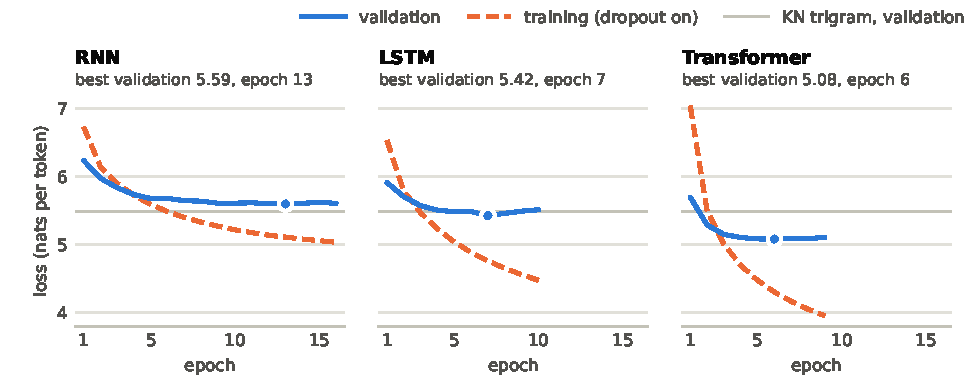
\includegraphics[width=\linewidth]{part1_loss_curves.pdf}
\caption{Training and validation loss per epoch. The dot marks the kept checkpoint; the grey line is the trigram's validation loss.}
\label{fig:part1curves}
\end{figure}

\paragraph{Generated text.} All models continue the same five prompts with temperature 0.8, top-$k$ 40 and 50 new tokens; the random generator is reset to the same seed for every continuation, and one sampling function serves all four models. Two examples, cut to their first 30 tokens (all samples: \tok{results/generations.json}):

\begin{small}
\begin{description}
\item[Prompt] \emph{the album was released in}
\item[KN trigram] the last game and the british empire casualties , " " and " the song . the ship 's cargo ship . the two \tok{<unk>} , \tok{<unk>} \tok{<unk>} , and \tok{<unk>} ( a ) \dots
\item[RNN] the 2000s season at the start of 14 august 1935 . a month of 3 : 10 , 2013 , also criticized a single film award for the game . the film \dots
\item[LSTM] the summer for three weeks of the uk and awards . in the episode in 2005 , the game was selected as the \tok{<unk>} \tok{<unk>} of the game 's best \dots
\item[Transformer] the united states . \tok{<eos>} in the album , in the united states on august 25 , 2015 , the album was released as a single album . the album received \dots
\item[Prompt] \emph{during the war , the}
\item[KN trigram] \tok{<unk>} , with a \tok{<unk>} " . however , due to an end . he has been a long time , the first half of the country , and the city , \dots
\item[RNN] 766th was a " \tok{<unk>} of the length , where no can be found for each of the first time . \tok{<eos>} the portuguese facade of the premaxillary \dots
\item[LSTM] \tok{<unk>} \tok{<unk>} were able to see the series of privacy that has been found at one of the same year . \tok{<eos>} the episode was directed by \dots
\item[Transformer] 766th was in order to create a heavy emplacement at about 20 km / h ( 11 mph ) . the 766th regiment 's regiment was made up to 40 km \dots
\end{description}
\end{small}

Across the five samples per model, the share of distinct bigrams is 0.94 for the trigram, 0.93 for the RNN, 0.94 for the LSTM and 0.90 for the Transformer, and the trigram produces the most \tok{<unk>} tokens (6.2 per 50-token sample, against 3.0 to 4.0); five samples are too few for small differences to mean much. Two facts worth noting: the trigram produced the identical continuation for ``the album was released in'' and ``the species is found in'' (both end in ``in'', both sampled ``the'' next, and from then on its two-token context and the random draws coincide), and the Transformer repeats ``766th'' three times within one sample. The trigram's samples are locally fluent over two or three words, but have no structure beyond that and do not stay on the prompt's topic. The RNN's are more fluent locally than the trigram's, but still lose the thread within a sentence or two and do not stay on topic. The LSTM's hold together slightly better over longer stretches, but are still not consistent with the prompt, most clearly for ``the species is found in''. The Transformer's are the most fluent both locally and across sentences. On repetition, the trigram is the clearest case: two different prompts led to an identical continuation. Among the neural models the Transformer repeats most, with the lowest share of distinct bigrams (0.90) and words such as ``album'', ``766th'' and ``chapel'' recurring within single samples.

\subsection{Tradeoffs}

\paragraph{Observed.} The trigram is far cheaper than any neural model to fit and to score known text, but its perplexity is behind the LSTM's and the Transformer's (and ahead of the RNN's). The LSTM has slightly more parameters than the RNN (24.2M against 21.5M) and costs the same per epoch, but reaches a lower perplexity and gains much more from longer history (Table~\ref{tab:context}). The Transformer has the fewest parameters and the lowest perplexity, trains fastest and is the fastest at inference: among the neural models on this setup there is no tradeoff, it is better on every axis measured. This holds for what was tested: WikiText-2, models of the sizes in Table~\ref{tab:arch}, a laptop's training budget and a single seed.

\paragraph{Possible explanations.} The LSTM's advantage over the RNN is consistent with its gating, which lets gradients and information pass across many steps without vanishing; the carried-state result, where the LSTM gains far more from long history than the RNN, points the same way. The Transformer's lead is consistent with its architecture: attention lets it see every earlier token in the window directly, instead of reading the context through a fixed-size recurrent state. Part of its lead comes from the start of each chunk (Figure~\ref{fig:byposition}), but not all of it: with that removed it is still well ahead (138.79 against 184.32 and 224.56, Table~\ref{tab:context}). The other candidates do not explain it: it has the fewest parameters, all models had the same 64-token context, and the training budget was the same apart from the learning-rate schedule.

\paragraph{Loss by amount of history.} Figure~\ref{fig:byposition} splits the test loss by position within the 64-token chunk, that is, by how many tokens of history each prediction had (\tok{results/analysis\_part1.json}). With one token of history the RNN and LSTM are far worse than both the Transformer and the trigram (perplexity 1,637 and 1,624, against 366 and 227). With more history all three neural models keep improving: from positions 8--15 to positions 32--63 their loss falls by 0.108 (RNN), 0.181 (LSTM) and 0.132 nats (Transformer), while the trigram's stays flat. Averaged over positions 32--63, the RNN is level with the trigram (perplexity 224 against 225), the LSTM is at 184 and the Transformer at 138. The poor start of the RNN and LSTM is a cold start. During training they carried their state from one batch to the next, so they almost never had to predict from a zero state, which is exactly how every evaluation chunk begins; the Transformer, which has no state, was trained and evaluated on chunks from scratch in the same way. A shortage of history alone does not explain it: with a single token of history the Transformer (366) and the trigram (227, always two tokens) do far better.

\begin{figure}[h]
\centering
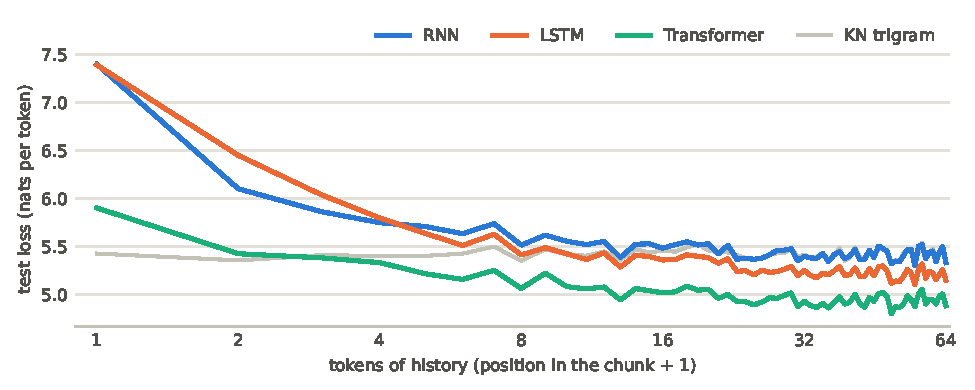
\includegraphics[width=\linewidth]{part1_loss_by_position.pdf}
\caption{Test loss by the number of tokens of history, for every position of a 64-token chunk (3,815 chunks). The trigram always has two tokens of history; its line is flat.}
\label{fig:byposition}
\end{figure}

\paragraph{Other ways of giving the models history.} Table~\ref{tab:context} scores the same test targets under two further protocols (\tok{results/analysis\_part1.json}). \emph{Strided}: windows of 64 tokens start every 32 tokens, each from a fresh state, and only their second half is scored, so every scored prediction has between 33 and 64 tokens of history and no model's slow start is counted. \emph{Carried}: the RNN and LSTM keep their state across the whole test stream, as in training, so their history is unlimited; the Transformer cannot do this, because it only ever attends to a fixed window.

\begin{table}[h]
\centering\small
\begin{tabular}{lrrr}
\toprule
Model & Standard (64-token chunks) & Strided (33--64 tokens of history) & Carried (unlimited history) \\
\midrule
KN trigram & 226.00 & 226.00 & 226.00 \\
RNN & 245.14 & 224.56 & 221.35 \\
LSTM & 210.84 & 184.32 & 165.82 \\
Transformer & 149.52 & 138.79 & -- \\
\bottomrule
\end{tabular}
\caption{Test perplexity of the same checkpoints under three evaluation protocols. The trigram always conditions on two tokens, so its score does not change.}
\label{tab:context}
\end{table}

With the slow start removed (strided), the RNN moves from behind the trigram to marginally ahead of it (224.56 against 226.00), and the ranking of the other models is unchanged. Given unlimited history (carried), the LSTM improves by a further 18.5 perplexity points, the RNN by 3.2. These results fit a vanishing-gradient explanation for the RNN rather than the LSTM: within the window the RNN gains least from extra history, and given unlimited history it improves by only 3.2 points, against 18.5 for the LSTM, whose gating lets information from far back survive. The Transformer keeps improving up to the end of its 64-token window; how it would behave beyond that was not measured. The standard protocol, fixed in the README in advance, remains the headline comparison; these are extra evidence.

% ---------------------------------------------------------------------------
\section{Part II: Embedding variants}
% ---------------------------------------------------------------------------

\subsection{Setup}

The LSTM from Part~I is trained with three input-embedding settings. Everything except the input embedding table is identical across them: architecture, embedding size (200), data, training procedure and random seed, so every other weight starts from the same value.

\begin{enumerate}
\item \textbf{Random, trainable.} The Part~I LSTM itself: a random table learned jointly with the model.
\item \textbf{Own skip-gram, frozen.} 200-dimensional skip-gram vectors trained with gensim on the WikiText-2 training split only (window 5, 10 negative samples, 10 epochs), one line per sentence. They cover every vocabulary token except \tok{<pad>}, which never occurs. Training them took 233\,s on the CPU, in addition to the language-model training.
\item \textbf{GloVe, frozen.} The public \tok{glove.6B.200d} vectors, trained on 6B tokens of Wikipedia and Gigaword. They cover 27,810 of the 28,913 vocabulary tokens (96.2\%), which make up 97.4\% of the training text. The most frequent missing tokens are \tok{<eos>} (23,767 occurrences in training) and the WikiText markers \tok{@-@}, \tok{@.@} and \tok{@,@}.
\end{enumerate}

In both frozen settings a token without a vector gets a row drawn from a normal distribution with mean 0 and the standard deviation of the vectors that were found, from a seeded generator. The \emph{entire} table, these rows included, is frozen; after training it was checked to be bit-for-bit unchanged. Freezing leaves 18.4M trainable parameters, against 24.2M in the random setting.

The settings are built to answer two questions. Settings 1 and 2 both learn their embeddings from the same WikiText-2 training text; they differ in whether the embeddings are learned jointly with the language model and kept trainable, or learned separately and then frozen. Settings 2 and 3 are both learned separately and frozen; they differ in the data the embeddings were trained on (2M WikiText tokens against 6B tokens of general text), and also in the method (skip-gram against GloVe), so this second comparison does not isolate the data alone.

\subsection{Results}

\begin{table}[h]
\centering\small
\begin{tabular}{lrrcccr}
\toprule
Input embeddings & Trainable params & Coverage & Val PPL & Test PPL & Epochs (best) & s / epoch \\
\midrule
Random, trainable & 24.2M & -- & 226.13 & 210.84 & 10 (7) & 480 \\
Own skip-gram, frozen & 18.4M & 100\% & 155.29 & \textbf{147.01} & 13 (10) & 452 \\
GloVe, frozen & 18.4M & 96.2\% & 178.42 & 167.55 & 13 (10) & 433 \\
\bottomrule
\end{tabular}
\caption{Part II results (\tok{results/lstm*.json}). Coverage is the share of vocabulary tokens with a pretrained vector. Time per epoch is measured as in Table~\ref{tab:part1}.}
\label{tab:part2}
\end{table}

\begin{figure}[h]
\centering
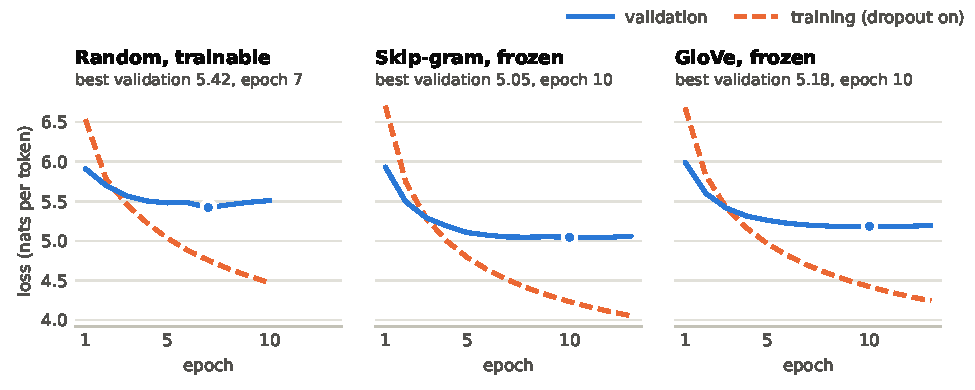
\includegraphics[width=\linewidth]{part2_loss_curves.pdf}
\caption{Training and validation loss per epoch for the three embedding settings. The dot marks the kept checkpoint.}
\label{fig:part2curves}
\end{figure}

\paragraph{Prediction quality.} Both frozen settings beat the random, trainable one by a wide margin: test perplexity 147.01 with the skip-gram vectors and 167.55 with GloVe, against 210.84. The frozen skip-gram LSTM is also slightly better than the Part~I Transformer (149.52).

\paragraph{Convergence and stability.} After one epoch the three settings are level (validation loss 5.91, 5.93 and 5.99). From the second epoch on, both frozen settings have the lower validation loss at every epoch, and they keep improving for longer: their best epoch is 10, against 7 for the random setting, whose validation loss then rises (Figure~\ref{fig:part2curves}). After the first epoch all three curves are smooth; the random setting's best epoch is a small dip (5.482, 5.421, 5.456 over epochs 6 to 8), while the frozen settings flatten out steadily. Per epoch, the frozen settings are slightly cheaper (452 and 433\,s against 480\,s), since the embedding table needs no gradient.

\paragraph{Generated text.} The same prompts and decoding as in Part~I (all samples: \tok{results/generations\_part2.json}). The random setting's samples tend not to stay on the prompt's topic; both frozen settings stay on topic more consistently (``the species is found in'' continues with genus, holotype and habitats under skip-gram, and with birds under GloVe). Local fluency is reasonable in all three and better in the frozen settings. On repetition, the frozen settings repeat more within a sample: their share of distinct bigrams is 0.92 (skip-gram) and 0.91 (GloVe) against 0.94 for the random setting, and the skip-gram sample for the species prompt uses ``species'' four times and ``genus'' three times. The GloVe setting produces the most \tok{<unk>} tokens (5.2 per sample, against 2.0 for skip-gram and 3.0 for random).

\subsection{Interpretation}

\paragraph{Trainability (settings 1 and 2).} Learning the embeddings separately and then freezing them helps here. One possible reason is stability: with a frozen table, the LSTM's inputs do not change during training, while in the random setting the embedding table and the rest of the model have to be learned at the same time from the same data, so the LSTM is fitted to inputs that keep moving. The frozen settings also overfit later and less, which is consistent with this: they reach their best epoch three epochs later, at a lower validation loss. \todo{Optional: whether having 5.8M fewer parameters to fit from the same 2M tokens also plays a part.}

\paragraph{Extra data (settings 2 and 3).} The skip-gram vectors were trained on the very corpus the language model is trained and tested on, so they match its vocabulary, tokenization and topics, while GloVe was trained on different text, tokenized differently. On this corpus that match outweighs the roughly 3,000 times more data GloVe saw. It also shows in coverage: GloVe has no vectors for \tok{<eos>} or the \tok{@-@}, \tok{@.@} and \tok{@,@} markers, some of the most frequent tokens in WikiText-2, so in the GloVe setting those tokens keep random, frozen rows that the model can never adapt. On a general corpus closer to GloVe's own training text, we would expect GloVe to do better than vectors trained on WikiText-2 alone; that was not tested here.

\paragraph{A confound: scale.} The three tables also start at different scales: the random table has standard deviation 1.0 (PyTorch's default), the skip-gram vectors 0.19 and GloVe 0.43. The initial scale matters in itself, so part of the gap between the random setting and the frozen ones may come from scale rather than from what the vectors contain. This experiment cannot separate the two; a random, trainable table started at the pretrained vectors' scale would.

% ---------------------------------------------------------------------------
\section{Part III: Downstream representations}
% ---------------------------------------------------------------------------

\subsection{Setup}

\paragraph{Task and data.} Topic classification on AG News (four balanced classes: World, Sports, Business, Sci/Tech; chance is 25\%). A class-balanced, seeded sample of 10,000 items from the official training split is used for training and a disjoint 2,000 for validation; the official test split (7,600) is used once. Each item (headline and summary) is lowercased, tokenized following WikiText-2's conventions and mapped to the WikiText-2 vocabulary, so the language models see it exactly as they would see their own data; 7.0\% of test tokens become \tok{<unk>}. Items are cut to 64 tokens, the chunk length the models were trained on; 3.8\% of test items are longer.

\paragraph{Representations.} Two frozen language models from Part~I, the LSTM and the Transformer, each read every item from a fresh state, and their final-layer hidden states (512 and 200 numbers per token) are collapsed into one vector per item in two ways: \emph{mean pooling}, the average of the hidden states over the item's real tokens, excluding padding; and \emph{last-token pooling}, the hidden state at the item's last real token, which has read the whole item. Both models read left to right, so the padding after an item cannot affect these states.

\paragraph{Classifier.} The same for all four representations: multinomial logistic regression on standardized features (standardization fitted on the training items only), with the regularization strength chosen by validation macro-F1 from $\{0.01, 0.1, 1, 10\}$. Only the classifier is trained; the language models stay frozen.

\subsection{Results}

\begin{table}[h]
\centering\small
\begin{tabular}{lrlrr}
\toprule
Language model & LM test PPL & Pooling & Test accuracy & Test macro-F1 \\
\midrule
LSTM & 210.84 & mean & 62.89\% & 0.628 \\
LSTM & 210.84 & last token & 47.62\% & 0.475 \\
Transformer & 149.52 & mean & \textbf{78.45\%} & \textbf{0.784} \\
Transformer & 149.52 & last token & 72.83\% & 0.727 \\
\bottomrule
\end{tabular}
\caption{Part III results (\tok{results/probe\_agnews.json}).}
\label{tab:part3}
\end{table}

\paragraph{Which representation works better.} The Transformer's representations beat the LSTM's with either pooling, and mean pooling beats last-token pooling for both models, by 15.3 points for the LSTM and 5.6 for the Transformer. The last real token of 84\% of test items is a full stop, so last-token pooling takes the state the model holds just after a sentence ends, when its job is mostly to predict what follows the end of a sentence rather than to describe what the item was about. The information that identifies the topic is spread over the item and is not guaranteed to be in that final state; averaging over every token keeps it.

The gap between the two poolings fits the same difference as in Part~I. In the LSTM, information from early in an item has to be carried through every later step to reach the final state, so the last state holds the beginning of the item only weakly. In the Transformer, the last position attends to every earlier token directly, without recurrence, so its final state loses less. The same holds for the states that mean pooling averages: each LSTM state summarizes all the history before it through one fixed-size state, while each Transformer state draws on the earlier tokens directly.

\paragraph{Errors.} Every probe finds Sports easiest and Business and Sci/Tech hardest (best probe: F1 0.89 for Sports, 0.80 World, 0.73 Sci/Tech, 0.71 Business), and its largest confusions are between Business and Sci/Tech (331 Business items predicted as Sci/Tech, 320 the other way). The ten most confident errors of each probe fall into three groups:
\begin{itemize}
\item \emph{Doubtful labels.} Sports stories labelled World are the most common confident error in every probe, for example ``Football: Azerbaijan 0-1 England. Michael Owen heads England's winner in the World Cup qualifier'' (labelled World, predicted Sports). These are arguably problems of the dataset, not of the model.
\item \emph{Genuinely ambiguous topics.} ``How Serious Is Pfizer's Condition? The stock is feeling some pain these days'' (Business, predicted Sci/Tech) and ``Treo 650 on Monday? The blogs are buzzing that the Treo 650 will be released'' (Sci/Tech, predicted Business) could each reasonably belong to either class.
\item \emph{Model errors.} ``Calif.\ Lawmaker Wants to Privatize State Pensions'' (Business) is predicted as Sports with full confidence by the Transformer with last-token pooling.
\end{itemize}

One possible contributor to the Business and Sci/Tech confusion is unknown words, since both classes are full of company and product names that WikiText-2 does not contain. The data give this only weak support: Sci/Tech has the highest \tok{<unk>} rate (8.2\% of tokens, against 6.2\% for World), but Business (7.0\%) is no higher than Sports (7.0\%); in the best probe, Business items predicted as Sci/Tech contain slightly more \tok{<unk>} than correctly classified ones (7.8\% against 7.0\%), and Sci/Tech items predicted as Business hardly more (8.4\% against 8.3\%); in the two LSTM probes, Sci/Tech items predicted as Business contain \emph{fewer} \tok{<unk>} than correctly classified ones. A more likely explanation is ambiguity in the task itself. Much news sits between the two classes: a technology company's earnings, for example, is as much Business as Sci/Tech, and which one it gets depends on the labelling. Each item carries a single hard label, not a distribution over classes, so the dataset has no way to say ``somewhere in between'', and items of this kind will be confused whichever representation is used.

\paragraph{Language-model ranking against downstream ranking.} The rankings agree: the Transformer, with the lower perplexity, also gives the better features, under both poolings. With only two language models this is a single comparison, not a trend; the frozen skip-gram LSTM from Part~II, which has a lower perplexity than either (147.01), was not probed. Better next-token prediction does not in general guarantee better features for another task, and this experiment cannot show how strongly the two are linked.

% ---------------------------------------------------------------------------
\section{Limitations and lessons}
% ---------------------------------------------------------------------------
\todo{Single seed; models not matched in size and not tuned; one laptop, timed in one power state; RNN/LSTM history capped at 64 tokens at evaluation; the PyTorch LSTM dropout bug and how it was caught.}

% ---------------------------------------------------------------------------
\section*{Tool use}
% ---------------------------------------------------------------------------
\todo{Your statement, consistent with the README's ``Tool use'' section.}

\end{document}
